%%%%%%%%%%%%%%%%%%%%%%%
% Comp 160, Fall 2019
% Homework 7
% Author: Vladimir Hugec
%%%%%%%%%%%%%%%%%%%%%%%

% This portion of the LaTeX document are configuration 
% You can see it as all the #includes in C++
\documentclass[12pt]{article}

\usepackage{epsfig}
\usepackage{amsmath}
\usepackage{amsthm}
\usepackage{listings}
\usepackage{graphicx}
\usepackage{tikz}

\newtheorem{lemma}{Lemma}
\newtheorem{theorem}{Theorem}

\usepackage{titlesec}
\titleformat{\section}
{\normalfont\Large\bfseries}{Question~\thesection:}{1em}{}

\newlength{\toppush}
\setlength{\toppush}{2\headheight}
\addtolength{\toppush}{\headsep}

\def\subjnum{Comp 160}
\def\subjname{Introduction to Algorithms}

\def\doheading#1#2#3{\vfill\eject\vspace*{-\toppush}%
  \vbox{\hbox to\textwidth{{\bf} \subjnum: \subjname \hfil Vladimir Hugec}%
    \hbox to\textwidth{{\bf} Tufts University, Fall 2019 \hfil#3\strut}%
    \hrule}}


\newcommand{\htitle}[1]{\vspace*{1.25ex plus 1ex minus 0ex}%
\begin{center}
{\large\bf #1}
\end{center}} 


%%%%%%%%%%%%%%%%%%%%%%%%%%%%%%%%%%%%%%%%%%%%%%%%%%%%%%%%%%%%%%%%%%%
% BEGIN DOCUMENT
%%%%%%%%%%%%%%%%%%%%%%%%%%%%%%%%%%%%%%%%%%%%%%%%%%%%%%%%%%%%%%%%%%%
\begin{document}
\doheading{2}{title}{Homework 7}

\section{}

\subsection{A}

\begin{center}
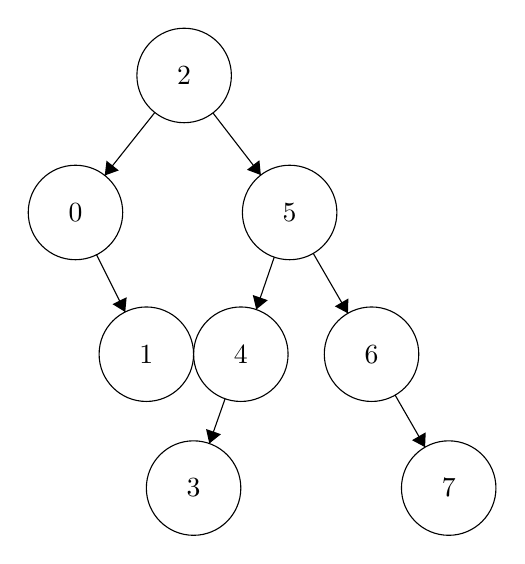
\begin{tikzpicture}[scale=0.2]
\tikzstyle{every node}+=[inner sep=0pt]
\draw [black] (37.9,-8) circle (3);
\draw (37.9,-8) node {$2$};
\draw [black] (44.6,-16.7) circle (3);
\draw (44.6,-16.7) node {$5$};
\draw [black] (31,-16.7) circle (3);
\draw (31,-16.7) node {$0$};
\draw [black] (35.5,-25.7) circle (3);
\draw (35.5,-25.7) node {$1$};
\draw [black] (41.5,-25.7) circle (3);
\draw (41.5,-25.7) node {$4$};
\draw [black] (49.8,-25.7) circle (3);
\draw (49.8,-25.7) node {$6$};
\draw [black] (54.7,-34.2) circle (3);
\draw (54.7,-34.2) node {$7$};
\draw [black] (38.5,-34.2) circle (3);
\draw (38.5,-34.2) node {$3$};
\draw [black] (36.04,-10.35) -- (32.86,-14.35);
\fill [black] (32.86,-14.35) -- (33.75,-14.03) -- (32.97,-13.41);
\draw [black] (32.34,-19.38) -- (34.16,-23.02);
\fill [black] (34.16,-23.02) -- (34.25,-22.08) -- (33.35,-22.52);
\draw [black] (39.73,-10.38) -- (42.77,-14.32);
\fill [black] (42.77,-14.32) -- (42.68,-13.38) -- (41.89,-13.99);
\draw [black] (43.62,-19.54) -- (42.48,-22.86);
\fill [black] (42.48,-22.86) -- (43.21,-22.27) -- (42.26,-21.94);
\draw [black] (46.1,-19.3) -- (48.3,-23.1);
\fill [black] (48.3,-23.1) -- (48.33,-22.16) -- (47.47,-22.66);
\draw [black] (51.3,-28.3) -- (53.2,-31.6);
\fill [black] (53.2,-31.6) -- (53.24,-30.66) -- (52.37,-31.16);
\draw [black] (40.5,-28.53) -- (39.5,-31.37);
\fill [black] (39.5,-31.37) -- (40.24,-30.78) -- (39.29,-30.45);
\end{tikzpicture}
\end{center}

\subsection{B}

Left-rotation on 5:

\begin{center}
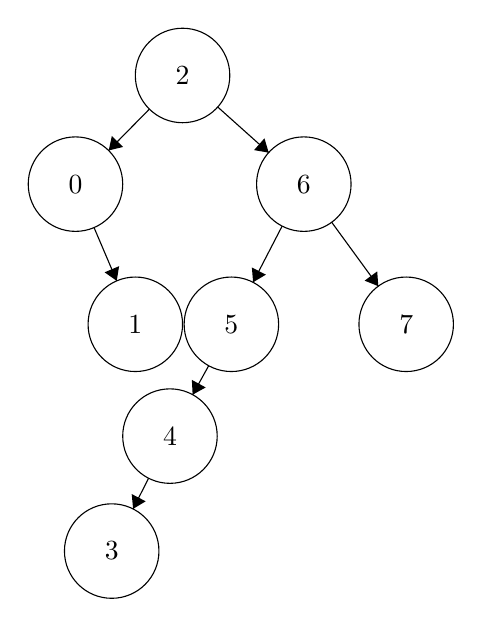
\begin{tikzpicture}[scale=0.2]
\tikzstyle{every node}+=[inner sep=0pt]
\draw [black] (33.6,-10.7) circle (3);
\draw (33.6,-10.7) node {$2$};
\draw [black] (32.8,-33.6) circle (3);
\draw (32.8,-33.6) node {$4$};
\draw [black] (26.8,-17.6) circle (3);
\draw (26.8,-17.6) node {$0$};
\draw [black] (30.6,-26.5) circle (3);
\draw (30.6,-26.5) node {$1$};
\draw [black] (29.1,-40.9) circle (3);
\draw (29.1,-40.9) node {$3$};
\draw [black] (36.7,-26.5) circle (3);
\draw (36.7,-26.5) node {$5$};
\draw [black] (41.3,-17.6) circle (3);
\draw (41.3,-17.6) node {$6$};
\draw [black] (47.8,-26.5) circle (3);
\draw (47.8,-26.5) node {$7$};
\draw [black] (31.49,-12.84) -- (28.91,-15.46);
\fill [black] (28.91,-15.46) -- (29.82,-15.24) -- (29.11,-14.54);
\draw [black] (27.98,-20.36) -- (29.42,-23.74);
\fill [black] (29.42,-23.74) -- (29.57,-22.81) -- (28.65,-23.2);
\draw [black] (31.44,-36.28) -- (30.46,-38.22);
\fill [black] (30.46,-38.22) -- (31.26,-37.74) -- (30.37,-37.28);
\draw [black] (35.26,-29.13) -- (34.24,-30.97);
\fill [black] (34.24,-30.97) -- (35.07,-30.51) -- (34.19,-30.03);
\draw [black] (43.07,-20.02) -- (46.03,-24.08);
\fill [black] (46.03,-24.08) -- (45.96,-23.14) -- (45.16,-23.73);
\draw [black] (35.83,-12.7) -- (39.07,-15.6);
\fill [black] (39.07,-15.6) -- (38.8,-14.69) -- (38.14,-15.44);
\draw [black] (39.92,-20.27) -- (38.08,-23.83);
\fill [black] (38.08,-23.83) -- (38.89,-23.35) -- (38,-22.89);
\end{tikzpicture}
\end{center}

Followed by a left-rotation on 2 = $T'$: 

\begin{center}
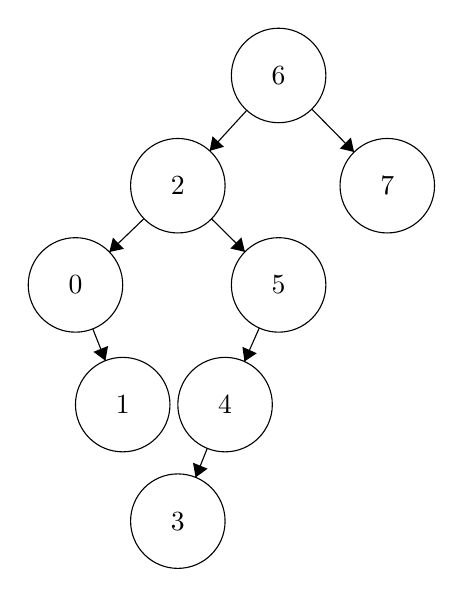
\begin{tikzpicture}[scale=0.2]
\tikzstyle{every node}+=[inner sep=0pt]
\draw [black] (33.3,-14.7) circle (3);
\draw (33.3,-14.7) node {$2$};
\draw [black] (36.3,-28.6) circle (3);
\draw (36.3,-28.6) node {$4$};
\draw [black] (26.8,-21) circle (3);
\draw (26.8,-21) node {$0$};
\draw [black] (29.8,-28.6) circle (3);
\draw (29.8,-28.6) node {$1$};
\draw [black] (33.3,-36) circle (3);
\draw (33.3,-36) node {$3$};
\draw [black] (39.7,-21) circle (3);
\draw (39.7,-21) node {$5$};
\draw [black] (39.7,-7.7) circle (3);
\draw (39.7,-7.7) node {$6$};
\draw [black] (46.6,-14.7) circle (3);
\draw (46.6,-14.7) node {$7$};
\draw [black] (31.15,-16.79) -- (28.95,-18.91);
\fill [black] (28.95,-18.91) -- (29.88,-18.71) -- (29.18,-18);
\draw [black] (27.9,-23.79) -- (28.7,-25.81);
\fill [black] (28.7,-25.81) -- (28.87,-24.88) -- (27.94,-25.25);
\draw [black] (35.17,-31.38) -- (34.43,-33.22);
\fill [black] (34.43,-33.22) -- (35.19,-32.67) -- (34.26,-32.29);
\draw [black] (38.47,-23.74) -- (37.53,-25.86);
\fill [black] (37.53,-25.86) -- (38.31,-25.34) -- (37.4,-24.93);
\draw [black] (41.81,-9.84) -- (44.49,-12.56);
\fill [black] (44.49,-12.56) -- (44.29,-11.64) -- (43.58,-12.34);
\draw [black] (35.44,-16.8) -- (37.56,-18.9);
\fill [black] (37.56,-18.9) -- (37.34,-17.98) -- (36.64,-18.69);
\draw [black] (37.68,-9.91) -- (35.32,-12.49);
\fill [black] (35.32,-12.49) -- (36.23,-12.23) -- (35.5,-11.56);
\end{tikzpicture}
\end{center}

\subsection{Red-Black $T$}

\begin{center}
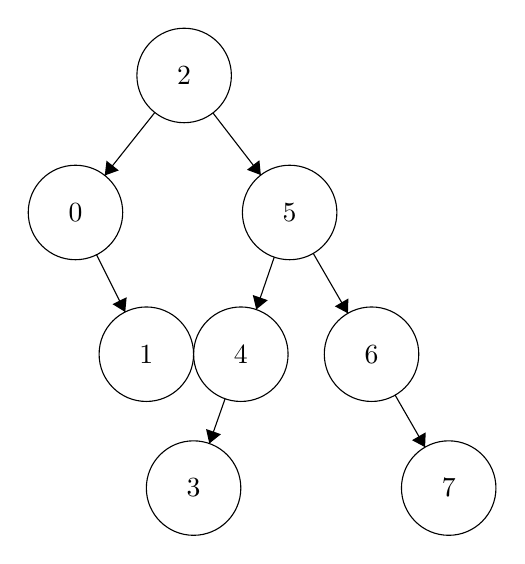
\begin{tikzpicture}[scale=0.2]
\tikzstyle{every node}+=[inner sep=0pt]
\draw [black] (37.9,-8) circle (3);
\draw (37.9,-8) node {$2$};
\draw [black] (44.6,-16.7) circle (3);
\draw (44.6,-16.7) node {$5$};
\draw [black] (31,-16.7) circle (3);
\draw (31,-16.7) node {$0$};
\draw [black] (35.5,-25.7) circle (3);
\draw (35.5,-25.7) node {$1$};
\draw [black] (41.5,-25.7) circle (3);
\draw (41.5,-25.7) node {$4$};
\draw [black] (49.8,-25.7) circle (3);
\draw (49.8,-25.7) node {$6$};
\draw [black] (54.7,-34.2) circle (3);
\draw (54.7,-34.2) node {$7$};
\draw [black] (38.5,-34.2) circle (3);
\draw (38.5,-34.2) node {$3$};
\draw [black] (36.04,-10.35) -- (32.86,-14.35);
\fill [black] (32.86,-14.35) -- (33.75,-14.03) -- (32.97,-13.41);
\draw [black] (32.34,-19.38) -- (34.16,-23.02);
\fill [black] (34.16,-23.02) -- (34.25,-22.08) -- (33.35,-22.52);
\draw [black] (39.73,-10.38) -- (42.77,-14.32);
\fill [black] (42.77,-14.32) -- (42.68,-13.38) -- (41.89,-13.99);
\draw [black] (43.62,-19.54) -- (42.48,-22.86);
\fill [black] (42.48,-22.86) -- (43.21,-22.27) -- (42.26,-21.94);
\draw [black] (46.1,-19.3) -- (48.3,-23.1);
\fill [black] (48.3,-23.1) -- (48.33,-22.16) -- (47.47,-22.66);
\draw [black] (51.3,-28.3) -- (53.2,-31.6);
\fill [black] (53.2,-31.6) -- (53.24,-30.66) -- (52.37,-31.16);
\draw [black] (40.5,-28.53) -- (39.5,-31.37);
\fill [black] (39.5,-31.37) -- (40.24,-30.78) -- (39.29,-30.45);
\end{tikzpicture}
\end{center}

\subsection{Red-Black $T'$}

\begin{center}
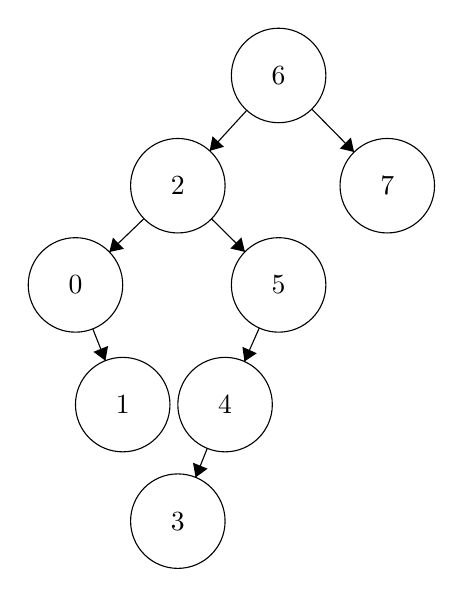
\begin{tikzpicture}[scale=0.2]
\tikzstyle{every node}+=[inner sep=0pt]
\draw [black] (33.3,-14.7) circle (3);
\draw (33.3,-14.7) node {$2$};
\draw [black] (36.3,-28.6) circle (3);
\draw (36.3,-28.6) node {$4$};
\draw [black] (26.8,-21) circle (3);
\draw (26.8,-21) node {$0$};
\draw [black] (29.8,-28.6) circle (3);
\draw (29.8,-28.6) node {$1$};
\draw [black] (33.3,-36) circle (3);
\draw (33.3,-36) node {$3$};
\draw [black] (39.7,-21) circle (3);
\draw (39.7,-21) node {$5$};
\draw [black] (39.7,-7.7) circle (3);
\draw (39.7,-7.7) node {$6$};
\draw [black] (46.6,-14.7) circle (3);
\draw (46.6,-14.7) node {$7$};
\draw [black] (31.15,-16.79) -- (28.95,-18.91);
\fill [black] (28.95,-18.91) -- (29.88,-18.71) -- (29.18,-18);
\draw [black] (27.9,-23.79) -- (28.7,-25.81);
\fill [black] (28.7,-25.81) -- (28.87,-24.88) -- (27.94,-25.25);
\draw [black] (35.17,-31.38) -- (34.43,-33.22);
\fill [black] (34.43,-33.22) -- (35.19,-32.67) -- (34.26,-32.29);
\draw [black] (38.47,-23.74) -- (37.53,-25.86);
\fill [black] (37.53,-25.86) -- (38.31,-25.34) -- (37.4,-24.93);
\draw [black] (41.81,-9.84) -- (44.49,-12.56);
\fill [black] (44.49,-12.56) -- (44.29,-11.64) -- (43.58,-12.34);
\draw [black] (35.44,-16.8) -- (37.56,-18.9);
\fill [black] (37.56,-18.9) -- (37.34,-17.98) -- (36.64,-18.69);
\draw [black] (37.68,-9.91) -- (35.32,-12.49);
\fill [black] (35.32,-12.49) -- (36.23,-12.23) -- (35.5,-11.56);
\end{tikzpicture}
\end{center}

Coloring this tree red black is not possible since because of the (5,4,3) subtree you cannot color it so that the all the lengths from root-to-nil nodes contain the same number of black nodes.

\pagebreak

\section{}

\subsection{A}

You are not guaranteed to be able to balance the tree if you allow for duplicates. For example: 

\begin{center}
\begin{tikzpicture}[scale=0.2]
\tikzstyle{every node}+=[inner sep=0pt]
\draw [black] (38.5,-10) circle (3);
\draw (38.5,-10) node {$5$};
\draw [black] (31.6,-18) circle (3);
\draw (31.6,-18) node {$5$};
\draw [black] (24.6,-26) circle (3);
\draw (24.6,-26) node {$5$};
\draw [black] (17.9,-33.6) circle (3);
\draw (17.9,-33.6) node {$5$};
\draw [black] (36.54,-12.27) -- (33.56,-15.73);
\fill [black] (33.56,-15.73) -- (34.46,-15.45) -- (33.7,-14.8);
\draw [black] (29.62,-20.26) -- (26.58,-23.74);
\fill [black] (26.58,-23.74) -- (27.48,-23.47) -- (26.73,-22.81);
\draw [black] (22.62,-28.25) -- (19.88,-31.35);
\fill [black] (19.88,-31.35) -- (20.79,-31.08) -- (20.04,-30.42);
\end{tikzpicture}
\end{center}

The tree is not balanced, and any attempts to balance the tree would invalidate the premise that all values that are equal to the parent are left side children. That being said, this does not mean that all tree's that allow for these duplicates cannot be balanced, just that you are not guaranteed to be able to.

\subsection{B}

Since by definition of our structure we know that duplicate items must be left side children of the desired value, we can eliminate searching the right side in our algorithm in the first case, in all subsequent levels both sides must be searched. The algorithm is as follows:

\pagebreak
		
$\newline$FUNCTION findAllOccurances (POINTER BSTnode, value, POINTER count)
	
LOOP while BSTnode is not NULL

$\indent$ IF value at node in BST equals our desired value

			$\indent \indent$increment count by one
			
			$\indent \indent$recursivly call findAllOccurances on left subtree
			
		$\indent$ ELSE IF value at node in BST is greater than our desired value
		
				$\indent \indent$ recursivly call findAllOccurances on left subtree
				
		$\indent$ ELSE IF value at node in BST is less than our desired value
		
				$\indent \indent$ recursivly call findAllOccurances on right subtree
				
		$\indent$ END-IF
		
END-LOOP
				
$\indent$ RETURN count

END-FUNCTION

\subsection{C}

This algorithm is correct since it recursively goes through each possible spot a duplicate of the desired value can be found. If the duplicate value we are looking for is found, then all subsequent duplicates must be a left child of that node. At the next level, if the node, now our relative root, is not the desired value, then it is compared to the value and based on that comparison, either the left or right subtree is recursed on.

\subsection{D}

Since we know that we are never recursing on more than one side of a node at any point, at each recursive call we are effectively cutting the search space in half. If we start with $n$ elements in the BST, and at each recursive call we narrow the possible landing spot of a duplicate by half we can say with reasonable certainty, assuming that the comparisons at each level run in constant time, that the algorithm would then be $O($log $n)$.

\pagebreak

\section{}

\subsection{A}

In this case, insert black $x$ as left child of $p(x)$. If this addition violates that rule that all routes from root to leaf (NIL) are equal, recolor $x$ red.

\begin{center}
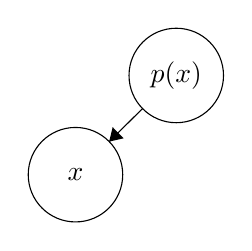
\begin{tikzpicture}[scale=0.2]
\tikzstyle{every node}+=[inner sep=0pt]
\draw [black] (37.5,-12.8) circle (3);
\draw (37.5,-12.8) node {$p(x)$};
\draw [black] (31.1,-19.1) circle (3);
\draw (31.1,-19.1) node {$x$};
\draw [black] (35.36,-14.9) -- (33.24,-17);
\fill [black] (33.24,-17) -- (34.16,-16.79) -- (33.46,-16.08);
\end{tikzpicture}

If violation occurs: $\downarrow$ 

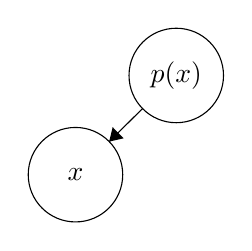
\begin{tikzpicture}[scale=0.2]
\tikzstyle{every node}+=[inner sep=0pt]
\draw [black] (37.5,-12.8) circle (3);
\draw (37.5,-12.8) node {$p(x)$};
\draw [black] (31.1,-19.1) circle (3);
\draw (31.1,-19.1) node {$x$};
\draw [black] (35.36,-14.9) -- (33.24,-17);
\fill [black] (33.24,-17) -- (34.16,-16.79) -- (33.46,-16.08);
\end{tikzpicture}
\end{center}

	
\subsection{B}

In this case, insert black $x$ as left child of $p(x)$. If this addition violates that rule that all routes from root to leaf (NIL) are equal, recolor $x$ red.

\begin{center}
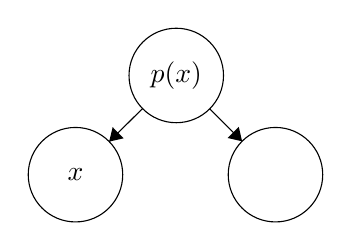
\begin{tikzpicture}[scale=0.2]
\tikzstyle{every node}+=[inner sep=0pt]
\draw [black] (37.5,-12.8) circle (3);
\draw (37.5,-12.8) node {$p(x)$};
\draw [black] (31.1,-19.1) circle (3);
\draw (31.1,-19.1) node {$x$};
\draw [black] (43.8,-19.1) circle (3);
\draw [black] (35.36,-14.9) -- (33.24,-17);
\fill [black] (33.24,-17) -- (34.16,-16.79) -- (33.46,-16.08);
\draw [black] (39.62,-14.92) -- (41.68,-16.98);
\fill [black] (41.68,-16.98) -- (41.47,-16.06) -- (40.76,-16.77);
\end{tikzpicture}

If violation occurs: $\downarrow$ 

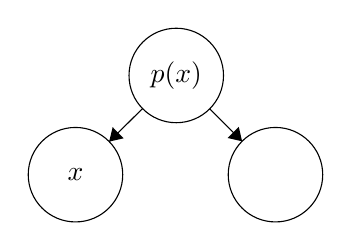
\begin{tikzpicture}[scale=0.2]
\tikzstyle{every node}+=[inner sep=0pt]
\draw [black] (37.5,-12.8) circle (3);
\draw (37.5,-12.8) node {$p(x)$};
\draw [black] (31.1,-19.1) circle (3);
\draw (31.1,-19.1) node {$x$};
\draw [black] (43.8,-19.1) circle (3);
\draw [black] (35.36,-14.9) -- (33.24,-17);
\fill [black] (33.24,-17) -- (34.16,-16.79) -- (33.46,-16.08);
\draw [black] (39.62,-14.92) -- (41.68,-16.98);
\fill [black] (41.68,-16.98) -- (41.47,-16.06) -- (40.76,-16.77);
\end{tikzpicture}
\end{center}

\subsection{C}

In this case, simply insert black $x$ as left child of $p(x)$.

\begin{center}
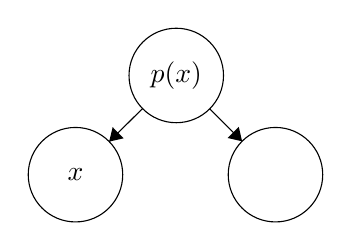
\begin{tikzpicture}[scale=0.2]
\tikzstyle{every node}+=[inner sep=0pt]
\draw [black] (37.5,-12.8) circle (3);
\draw (37.5,-12.8) node {$p(x)$};
\draw [black] (31.1,-19.1) circle (3);
\draw (31.1,-19.1) node {$x$};
\draw [black] (43.8,-19.1) circle (3);
\draw [black] (35.36,-14.9) -- (33.24,-17);
\fill [black] (33.24,-17) -- (34.16,-16.79) -- (33.46,-16.08);
\draw [black] (39.62,-14.92) -- (41.68,-16.98);
\fill [black] (41.68,-16.98) -- (41.47,-16.06) -- (40.76,-16.77);
\end{tikzpicture}

If violation occurs: $\downarrow$ 

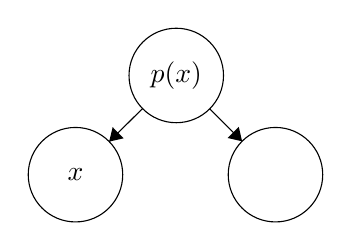
\begin{tikzpicture}[scale=0.2]
\tikzstyle{every node}+=[inner sep=0pt]
\draw [black] (37.5,-12.8) circle (3);
\draw (37.5,-12.8) node {$p(x)$};
\draw [black] (31.1,-19.1) circle (3);
\draw (31.1,-19.1) node {$x$};
\draw [black] (43.8,-19.1) circle (3);
\draw [black] (35.36,-14.9) -- (33.24,-17);
\fill [black] (33.24,-17) -- (34.16,-16.79) -- (33.46,-16.08);
\draw [black] (39.62,-14.92) -- (41.68,-16.98);
\fill [black] (41.68,-16.98) -- (41.47,-16.06) -- (40.76,-16.77);
\end{tikzpicture}
\end{center}

\subsection{D}

In this case, simply insert black $x$ as left child of $p(x)$. If this addition violates that rule that all routes from root to leaf (NIL) are equal, recolor $x$ red and $p(x)$ black. If  $p(x)$ is the root, also recolor $p(x)$ black and $x$ red.

\begin{center}
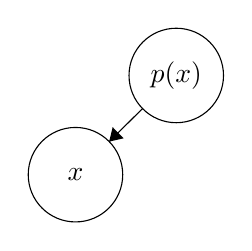
\begin{tikzpicture}[scale=0.2]
\tikzstyle{every node}+=[inner sep=0pt]
\draw [black] (37.5,-12.8) circle (3);
\draw (37.5,-12.8) node {$p(x)$};
\draw [black] (31.1,-19.1) circle (3);
\draw (31.1,-19.1) node {$x$};
\draw [black] (35.36,-14.9) -- (33.24,-17);
\fill [black] (33.24,-17) -- (34.16,-16.79) -- (33.46,-16.08);
\end{tikzpicture}

If violation occurs: $\downarrow$ 

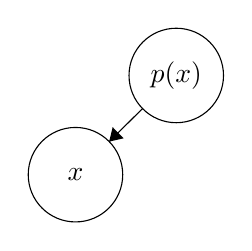
\begin{tikzpicture}[scale=0.2]
\tikzstyle{every node}+=[inner sep=0pt]
\draw [black] (37.5,-12.8) circle (3);
\draw (37.5,-12.8) node {$p(x)$};
\draw [black] (31.1,-19.1) circle (3);
\draw (31.1,-19.1) node {$x$};
\draw [black] (35.36,-14.9) -- (33.24,-17);
\fill [black] (33.24,-17) -- (34.16,-16.79) -- (33.46,-16.08);
\end{tikzpicture}
\end{center}

\subsection{E}

In this case, insert black $x$ as left child of $p(x)$. The sibling of $x$ violates the rule that children of a red-parent must be black, recolor $x$'s sibling black. If on the other-hand $p(x)$ is the root, recolor $p(x)$ black then both $x$ and its' sibling red.

\begin{center}
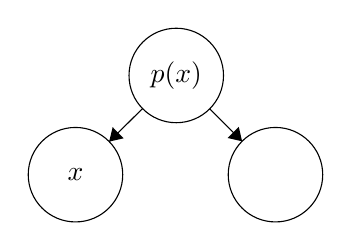
\begin{tikzpicture}[scale=0.2]
\tikzstyle{every node}+=[inner sep=0pt]
\draw [black] (37.5,-12.8) circle (3);
\draw (37.5,-12.8) node {$p(x)$};
\draw [black] (31.1,-19.1) circle (3);
\draw (31.1,-19.1) node {$x$};
\draw [black] (43.8,-19.1) circle (3);
\draw [black] (35.36,-14.9) -- (33.24,-17);
\fill [black] (33.24,-17) -- (34.16,-16.79) -- (33.46,-16.08);
\draw [black] (39.62,-14.92) -- (41.68,-16.98);
\fill [black] (41.68,-16.98) -- (41.47,-16.06) -- (40.76,-16.77);
\end{tikzpicture}

$\downarrow$ 

$\newline$

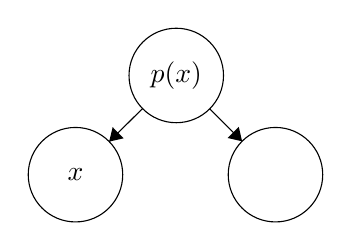
\begin{tikzpicture}[scale=0.2]
\tikzstyle{every node}+=[inner sep=0pt]
\draw [black] (37.5,-12.8) circle (3);
\draw (37.5,-12.8) node {$p(x)$};
\draw [black] (31.1,-19.1) circle (3);
\draw (31.1,-19.1) node {$x$};
\draw [black] (43.8,-19.1) circle (3);
\draw [black] (35.36,-14.9) -- (33.24,-17);
\fill [black] (33.24,-17) -- (34.16,-16.79) -- (33.46,-16.08);
\draw [black] (39.62,-14.92) -- (41.68,-16.98);
\fill [black] (41.68,-16.98) -- (41.47,-16.06) -- (40.76,-16.77);
\end{tikzpicture}

If root violation occurs: $\downarrow$ 

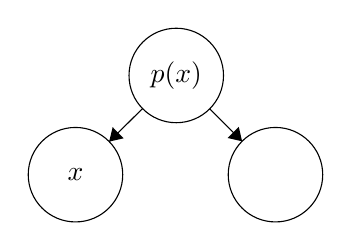
\begin{tikzpicture}[scale=0.2]
\tikzstyle{every node}+=[inner sep=0pt]
\draw [black] (37.5,-12.8) circle (3);
\draw (37.5,-12.8) node {$p(x)$};
\draw [black] (31.1,-19.1) circle (3);
\draw (31.1,-19.1) node {$x$};
\draw [black] (43.8,-19.1) circle (3);
\draw [black] (35.36,-14.9) -- (33.24,-17);
\fill [black] (33.24,-17) -- (34.16,-16.79) -- (33.46,-16.08);
\draw [black] (39.62,-14.92) -- (41.68,-16.98);
\fill [black] (41.68,-16.98) -- (41.47,-16.06) -- (40.76,-16.77);
\end{tikzpicture}
\end{center}

\subsection{F}

In this case, insert black $x$ as left child of $p(x)$. If  $p(x)$ is the root, recolor $p(x)$ black, and both $x$ and its' sibling red.

\begin{center}
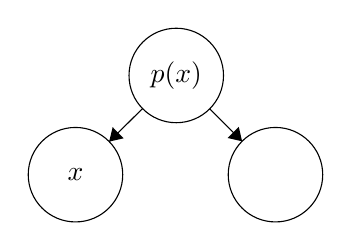
\begin{tikzpicture}[scale=0.2]
\tikzstyle{every node}+=[inner sep=0pt]
\draw [black] (37.5,-12.8) circle (3);
\draw (37.5,-12.8) node {$p(x)$};
\draw [black] (31.1,-19.1) circle (3);
\draw (31.1,-19.1) node {$x$};
\draw [black] (43.8,-19.1) circle (3);
\draw [black] (35.36,-14.9) -- (33.24,-17);
\fill [black] (33.24,-17) -- (34.16,-16.79) -- (33.46,-16.08);
\draw [black] (39.62,-14.92) -- (41.68,-16.98);
\fill [black] (41.68,-16.98) -- (41.47,-16.06) -- (40.76,-16.77);
\end{tikzpicture}

If violation occurs: $\downarrow$ 

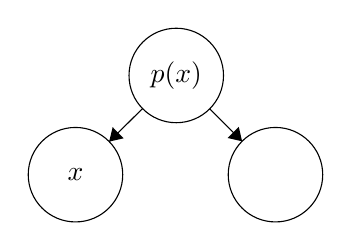
\begin{tikzpicture}[scale=0.2]
\tikzstyle{every node}+=[inner sep=0pt]
\draw [black] (37.5,-12.8) circle (3);
\draw (37.5,-12.8) node {$p(x)$};
\draw [black] (31.1,-19.1) circle (3);
\draw (31.1,-19.1) node {$x$};
\draw [black] (43.8,-19.1) circle (3);
\draw [black] (35.36,-14.9) -- (33.24,-17);
\fill [black] (33.24,-17) -- (34.16,-16.79) -- (33.46,-16.08);
\draw [black] (39.62,-14.92) -- (41.68,-16.98);
\fill [black] (41.68,-16.98) -- (41.47,-16.06) -- (40.76,-16.77);
\end{tikzpicture}
\end{center}

\end{document}
%%%%%%%%%%%%%%%%%%%%%%%%%%%%%%%%%%%%%%%%%%%%%%%%%%%%%%%%%%%%%%%%%%%%%%

